%\documentclass[german,10pt]{book}      
\usepackage{makeidx}
\usepackage{babel}            % Sprachunterstuetzung
\usepackage{amsmath}          % AMS "Grundpaket"
\usepackage{amssymb,amsfonts,amsthm,amscd} 
\usepackage{mathrsfs}
\usepackage{rotating}
\usepackage{sidecap}
\usepackage{graphicx}
\usepackage{color}
\usepackage{fancybox}
\usepackage{tikz}
\usetikzlibrary{arrows,snakes,backgrounds}
\usepackage{hyperref}
\hypersetup{colorlinks=true,
                    linkcolor=blue,
                    filecolor=magenta,
                    urlcolor=cyan,
                    pdftitle={Overleaf Example},
                    pdfpagemode=FullScreen,}
%\newcommand{\hyperref}[1]{\ref{#1}}
%
\definecolor{Gray}{gray}{0.80}
\DeclareMathSymbol{,}{\mathord}{letters}{"3B}
%
\newcounter{num}
\renewcommand{\thenum}{\arabic{num}}
\newenvironment{anmerkungen}
   {\begin{list}{(\thenum)}{%
   \usecounter{num}%
   \leftmargin0pt
   \itemindent5pt
   \topsep0pt
   \labelwidth0pt}%
   }{\end{list}}
%
\renewcommand{\arraystretch}{1.15}                % in Formeln und Tabellen   
\renewcommand{\baselinestretch}{1.15}                 % 1.15 facher
                                                      % Zeilenabst.
\newcommand{\Anmerkung}[1]{{\begin{footnotesize}#1 \end{footnotesize}}\\[0.2cm]}
\newcommand{\comment}[1]{}
\setlength{\parindent}{0em}           % Nicht einruecken am Anfang der Zeile 

\setlength{\textwidth}{15.4cm}
\setlength{\textheight}{23.0cm}
\setlength{\oddsidemargin}{1.0mm} 
\setlength{\evensidemargin}{-6.5mm}
\setlength{\topmargin}{-10mm} 
\setlength{\headheight}{0mm}
\newcommand{\identity}{{\bf 1}}
%
\newcommand{\vs}{\vspace{0.3cm}}
\newcommand{\noi}{\noindent}
\newcommand{\leer}{}

\newcommand{\engl}[1]{[\textit{#1}]}
\parindent 1.2cm
\sloppy

         \begin{document}  \setcounter{chapter}{6}


\chapter{Quantenradierer}
% Kap x
\label{chap_Quantenradierer}

\info{Thomas Filk}{27.03.2024}%
Quantenradierer\index{Quantenradierer|(} 
z\"ahlen zu der Gruppe der sogenannten \glqq verz\"ogerte Wahl\grqq-Experimenten
(delayed choice),\index{delayed choice}\index{verz\"ogerte Wahl, Experimente} 
bei denen die Entscheidung, welche von zwei komplement\"aren Gr\"o\ss en
gemessen werden soll, erst gef\"allt wird, nachdem die entscheidende Wechselwirkung zwischen dem
Quantensystem und einem Element seiner Umgebung bereits stattgefunden hat. In den meisten
F\"allen handelt es sich bei Quantenradierern um Abwandlungen des 
Doppelspaltexperiments, bei\index{Doppelspaltexperiment}\index{Welcher Weg-Information|(} 
denen die \glqq Welcher-Weg\grqq-Information zun\"achst vorhanden ist, dann aber durch
einen weiteren Quanteneffekt unwiderruflich wieder gel\"oscht werden kann. Die Entscheidung,
ob man die \glqq Welcher-Weg\grqq-Information abrufen oder sie endg\"ultig l\"oschen m\"ochte,
wird gef\"allt, nachdem beispielsweise ein Photon  den Doppelspalt durchquert hat. 

Es gibt verschiedene Versionen von Quantenradierern, die unterschiedliche Eigenschaften
von Photonen zur Speicherung der \glqq Welcher-Weg\grqq-Information nutzen. Die
\glqq klassische Version\grqq\ l\"asst sich auch mit gew\"ohnlichem Laserlicht durchf\"uhren und
im Rahmen einer klassischen Wellentheorie des Lichts und seiner Polarisationseigenschaften
beschreiben. Dieser Versuch wird auch gelegentlich in der Schule durchgef\"uhrt. Er ist nicht ganz
so spektakul\"ar wie andere Versionen des Quantenradierers, da bei ihm die Information wieder
gel\"oscht wird, bevor die Photonen auf einen Schirm treffen und dort, je nachdem ob die
\glqq Welcher-Weg\grqq-Information vorhanden ist oder nicht, ein Interferenzmuster zeigen.
Bei Experimenten mit Einzelphotonen kann man oft die \glqq Welcher-Weg\grqq-Information
abrufen, nachdem die Photonen bereits registriert wurden oder auf einen Schirm 
getroffen sind. Da zumindest
im Prinzip die \glqq Welcher-Weg\grqq-Information vorhanden ist, sieht man zun\"achst kein
Interferenzmuster. Man kann anschlie\ss end jedoch entscheiden, ob man die 
\glqq Welcher-Weg\grqq-Information l\"oschen m\"ochte oder nicht. Entscheidet man sich,
im Rahmen einer Messung die \glqq Welcher-Weg\grqq-Information endg\"ultig zu l\"oschen, kann man 
als Ergebnis dieser Messung eine andere Information erhalten, mit deren Hilfe man eine Postselektion 
der Photonenspuren auf dem Schirm vornehmen kann, sodass Interferenzmuster sichtbar werden.

W\"ahrend Einzelphoton-Experimente auf absehbare Zeit f\"ur Schulen noch zu kostspielig sind,
eignen sich die verschiedenen Einzelphoton-Quantenradierer als Gedankenexperimente 
sehr gut, um bei Sch\"uler*innen
das Gesp\"ur, wann \glqq Welcher-Weg\grqq-Information vorliegt und wann nicht, zu st\"arken.
F\"ur die Polarisationszust\"ande von Licht oder Einzelphotonen verwenden wir folgende
Darstellung:
\begin{eqnarray}
   \mbox{horizontale und vertikale Polarisation} & & |h\rangle , |v \rangle \\
   \mbox{lineare Polarisation unter } \pm 45^\circ & & |+\rangle , | - \rangle \\
   \mbox{rechts- bzw.\ linkszirkulare Polariation} & & |R\rangle , |L \rangle \, .
\end{eqnarray}

Eine Anmerkung zur Sprechweise: Sehr oft findet man bei Strahlteilern die Sprechweise
\glqq f\"ur das Photon gibt es nun zwei m\"ogliche Wege\grqq\ oder so \"ahnlich. Eigentlich
sollte man eher sagen \glqq der quantenmechanische Zustand, durch den das Photon hinter 
dem Strahlteiler beschrieben wird, hat nun zwei Anteile ...\grqq. Die Sprechweise von den
zwei m\"oglichen Wegen beruht auf der Darstellung quantenmechanischer Prozesse
als Summe \"uber alle M\"oglichkeiten 
(Feynman's Summation \"uber Wege),\index{Feynman's Summation \"uber Wege}
wobei jeder M\"oglichkeit eine Amplitude zugeschrieben wird und zur Berechnung der
Wahrscheinlichkeit das Absolutquadrat der Summe \"uber alle Amplituden zu nehmen ist. 
Wenn man die Regeln f\"ur die Bestimmung solcher Amplituden beachtet, kann die
Sprechweise bzw.\ die Darstellung als Summe \"uber alle M\"oglichkeiten sehr anschaulich
und hilfreich sein, aber man sollte sich des Feynman'schen Modells im Hintergrund bewusst sein.


\section{Der \glqq klassische\grqq\ Quantenradierer}

Das einfachste Modell eines Quantenradierers l\"asst sich sowohl mit Laserlicht als auch
mit Einzelphotonen durchf\"uhren. Au\ss erdem kann man den Effekt sowohl im 
Rahmen einer klassischen Wellentheorie\index{Quantenradierer!klassischer}
des Lichts und seiner Polarisationseigenschaften erkl\"aren als auch im Rahmen einer
quantentheoretischen Beschreibung von Einzelphotonen. Interessant und relevant ist in diesem
Zusammenhang, dass sich koh\"ahentes Laserlicht in mehrfacher Hinsicht sehr \"ahnlich verh\"alt
wie Einzelphotonen. Insbesondere gilt dies f\"ur koh\"arente Superpositionen.
Im Folgenden behandeln wir zun\"achst den klassischen Fall und die
klassische Erkl\"arung, anschlie\ss end betrachten wir die gleiche Situation f\"ur Einzelphotonen
und beschreiben sie ihm Rahmen des quantentheoretischen Formalismus. 

\subsection{Laserlicht und polarisierte elektrische Felder}

Laserlicht beschreiben wir klassisch durch ein linear polarisiertes elektrisches
Feld $\vec{E}$ einer festen Wellenl\"ange $\lambda$ (die zeitliche Abh\"angigkeit lassen wir
unber\"ucksichtigt; sie \"andert nichts an den folgenden \"Uberlegungen). 
Vertikal polarisiertes Laserlicht treffe auf einen Doppelspalt, wobei
sich hinter dem rechten Spalt ein Polarisationsfilter unter $+45^\circ$ und hinter dem
linken Spalt ein Polarisationsfilter unter $-45^\circ$ befinde. Unmittelbar hinter dem
Doppelspalt haben wir somit zwei linear polarisierte elektrische Felder, $\vec{E}^+_r(x)$ und
$\vec{E}^-_l(x)$, wobei sich $r$ und $l$ auf den rechten bzw.\ linken Spalt 
beziehen (siehe Abb.\ \ref{fig_DSklass}). 

Das Laserlicht ist nun markiert: Die beiden $\pm$-diagonalen Polarisationen zeigen
an, welcher Teil des Laserlichts durch den linken und welcher durch den rechten Spalt
getreten ist. Etwas weiter hinter dem Doppelspalt \"uberlagern sich die beiden elektrischen
Felder, wobei es zwischen dem $+$-polarisierten Anteil und dem $-$-polarisierten Anteil
eine Phasenverschiebung $\delta$ gibt, die von der jeweiligen Differenz in der optischen 
Wegl\"ange abh\"angt:
\begin{equation}
                  \vec{E}_{\rm ges}(x) = \vec{E}^-_l(x) + {\rm e}^{{\rm i}\delta} \vec{E}^+_r(x) 
\end{equation}

\begin{figure}[htb]
\begin{tikzpicture}
\foreach \x in {0,0.2,0.4,0.6,0.8}
\draw (5,\x) -- (9,\x);
\filldraw[fill=gray!20] (0,1) -- (6,1) -- (6,1.2) -- (0,1.2);
\filldraw[fill=gray!20] (6.3,1) -- (7.7,1) -- (7.7,1.2) -- (6.3,1.2) -- (6.3,1);
\filldraw[fill=gray!20] (14.3,1) -- (8.0,1) -- (8.0,1.2) -- (14.3,1.2);
\draw(5.9,1.2) rectangle +(0.5,0.5);
\draw (6.4,1.2) -- (5.9,1.7);
\draw(7.6,1.2) rectangle +(0.5,0.5);
\draw (7.6,1.2) -- (8.1,1.7);
  \draw (1,6) ellipse (0.3cm and 0.3cm);
  \draw[->] (1,6.3) -- (1.01,6.3);
  \draw[->] (1,5.7) -- (0.99,5.7);
  \draw (2,6) ellipse (0.36cm and 0.18cm);
  \draw[->] (2,6.18) -- (2.01,6.18);
  \draw[->] (2,5.82) -- (1.99,5.82);
  \draw[<->] (2.6,6) -- (3.4,6);
  \draw (4,6) ellipse (0.36cm and 0.18cm);
  \draw[->] (4,6.18) -- (3.99,6.18);
  \draw[->] (4,5.82) -- (4.01,5.82);
  \draw (5,6) ellipse (0.3cm and 0.3cm);
  \draw[->] (5.0,6.3) -- (4.99,6.3);
  \draw[->] (5,5.7) -- (5.01,5.7);
  \draw (6,6) ellipse (0.18cm and 0.36cm);
  \draw[->] (5.82,5.98) -- (5.82,5.97);
  \draw[->] (6.18,6.02) -- (6.18,6.03);
  \draw[<->] (7,5.6) -- (7,6.4);
  \draw (8,6) ellipse (0.18cm and 0.36cm);
  \draw[->] (7.82,6.02) -- (7.82,6.03);
  \draw[->] (8.18,5.98) -- (8.18,5.97);
  \draw (9,6) ellipse (0.3cm and 0.3cm);
  \draw[->] (9,6.3) -- (9.01,6.3);
  \draw[->] (9,5.7) -- (8.99,5.7);
  \draw (10,6) ellipse (0.36cm and 0.18cm);
  \draw[->] (10,6.18) -- (10.01,6.18);
  \draw[->] (10,5.82) -- (9.99,5.82);
  \draw[<->] (10.6,6) -- (11.4,6);
  \draw (12,6) ellipse (0.36cm and 0.18cm); 
  \draw[->] (12,6.18) -- (11.99,6.18);
  \draw[->] (12,5.82) -- (12.01,5.82);
  \draw (13,6) ellipse (0.3cm and 0.3cm);
  \draw[->] (13.0,6.3) -- (12.99,6.3);
  \draw[->] (13,5.7) -- (13.01,5.7);
\draw (0,5.3) node {$\delta=$}; 
\draw (1,5.3) node {$-\frac{3\pi}{2}$}; 
\draw (2,5.3) node {$-\frac{5\pi}{4}$}; 
\draw (3,5.3) node {$-\pi$}; 
\draw (4,5.3) node {$-\frac{3\pi}{4}$}; 
\draw (5,5.3) node {$-\frac{\pi}{2}$}; 
\draw (6,5.3) node {$-\frac{\pi}{4}$}; 
\draw (7,5.3) node {$0$}; 
\draw (8,5.3) node {$\frac{\pi}{4}$}; 
\draw (9,5.3) node {$\frac{\pi}{2}$}; 
\draw (10,5.3) node {$\frac{3\pi}{4}$}; 
\draw (11,5.3) node {$\pi$}; 
\draw (12,5.3) node {$\frac{5\pi}{4}$}; 
\draw (13,5.3) node {$\frac{3\pi}{2}$}; 
\draw (6.15,1.7) -- (10,6.0) -- (7.85,1.7);
\end{tikzpicture}
\caption{\label{fig_DSklass}%
Der klassische Radierer: Licht trifft auf einen Doppelspalt, hinter dem sich $\pm$-Polarisationsfilter
befinden. Dadurch wird der Lichtstrahl \glqq markiert\grqq. Je nach der Differenz in der optischen
Wegl\"ange \"uberlagern sich die beiden Anteile zu $h/v$-linear polarisiertem Licht oder 
rechts-links-zirkular polarisiertem Licht bzw.\ allgemeiner elliptisch polarisiertem Licht.} 
\end{figure}

Triff dieses Licht auf einen Schirm, beobachtet man kein Interferenzmuster. Im Rahmen der
klassischen Physik sagt man, dass Lichtanteile zu orthogonalen Polarisationen nicht
miteinander interferieren. Platzieren wir zwischen den Doppelspalt und den Schirm einen
Polarisationsfilter unter $+ 45^\circ$ oder $-45^\circ$, verringert sich die Intensit\"at um die
H\"alfte, es erscheint aber immer noch kein Interferenzmuster, weil in diesem Fall nur das
Licht von einem der Spalte durch den Filter hindurchtritt und auf den Schirm trifft. 

Platzieren wir jedoch zwischen Doppelspalt und Schirm einen Polarisationsfilter unter einer
$v$- oder $h$-Orientierung,
beobachtet man ein Interferenzmuster. Wie man in Abb.\ \ref{fig_DSklass} erkennt, treten in
regelm\"a\ss igen Abst\"anden auf dem Schirm nur horizontale bzw.\ nur vertikale Polarisationen
auf. Dies liegt daran, dass sich die horizontale bzw.\ vertikale Polarisation als Linearkombinaton
von $\pm$-diagonal polarisiertem Licht auffassen lassen:
\begin{equation}
             \vec{E}^{h/v}(x) = \frac{1}{\sqrt{2}} \big( \vec{E}^{+}(x) \pm \vec{E}^{-}(x) \big) \, .
\end{equation}
Ist der relative Phasenwinkel zwischen den beiden Anteilen $\delta=0$,
erhalten wir vertikal polarisiertes Licht, bei einem relativen Phasenwinkeln von $\pm \pi$ erhalten wir
horizontal polarisiertes Licht. Die Projektion der elliptischen Polarisationen auf einen $h$- oder $v$-Filter
ergibt entsprechend geringere Intensit\"aten und insgesamt beobachtet man Interferenzstreifen.

Die beiden Interferenzmuster zu einem $h$-Polarisationsfilter bzw.\ $v$-Polarisationsfilter
sind gleich, allerdings um eine halbe Phase versetzt:
Dort, wo bei der $v$-Orientierung die Maxima sind, liegen beim $h$-Filter die Minima und
umgekehrt. Insgesamt zeigt sich f\"ur die Intensit\"at (ohne Ber\"ucksichtigung des Beugungsmusters
der Einzelspalte, das streng genommen mit dem Beugungsmuster des Doppelspalts zu falten w\"are,
bei gen\"ugend schmalen Spalten im Vergleich zu ihrem Abstand aber vernachl\"assigbar ist) 
die Beziehung:
\begin{equation}
              I_{\rm ges} =   I_h + I_v = I ( \cos^2 \delta + \sin^2 \delta)   \, ,
\end{equation}
wobei $I_{h/v}$ die Intensit\"aten sind, die man bei Verwendung eines horizontalen bzw.\
vertikalen Polarisationsfilters zwischen Doppelspalt und Schirm findet. Die Phasenverschiebung
\begin{equation}
        \delta = \frac{\Delta x}{\lambda} \, {\rm mod}\, 2\pi
\end{equation}
($\Delta x$ der Wegl\"angenunterschied zwischen den beiden Teilstrahlen zu einem
bestimmten Punkt am Schirm) 
ist in eine Koordinate entlang des Schirms umzurechnen (eine rein geometrische
Beziehung zwischen dem Abstand Doppelspalt-Schirm, $L$, und der $x$-Koordinate entlang des 
Schirms: $x/L=\tan \delta$). 

Das Auftreten eines Interferenzmusters am Schirm kann man auch so deuten, dass keine
\glqq Welcher-Weg\grqq-Information vorhanden ist. Die \glqq Welcher-Weg\grqq-Information, die
unmittelbar hinter dem Doppelspalt durch die $\pm$-Polarisationsfilter dem Strahl mitgegeben
wurde, wurde durch den zweiten Polarisationsfilter ($h/v$) wieder gel\"oscht. Dem Licht hinter dem
$h/v$-Filter kann man nicht mehr entnehmen, ob es urspr\"unglich mal $+$- oder $-$-polarisiert war.
Ein \"ahnliches Ergebnis w\"urden wir erhalten, wenn wir statt der $h/v$-Polarisation des zweiten
Filters eine $L/R$-Polarisation (links- rechts-zirkular polarisiert) herausfiltern w\"urden. Auch in diesem
Fall w\"urde man ein Interferenzmuster beobachten (die beiden Muster zu einem $R$- bzw.\ einem 
$L$-Filter sind wieder um eine Phase von $180^\circ$ verschoben; relativ zu den $h/v$-Mustern findet
man eine Phasenverschiebung von $90^\circ$).

Da man im Prinzip den Filter, den man zus\"atzlich vor den Schirm bringt, w\"ahlen kann, nachdem
das Licht durch den Doppelspalt getreten ist, spricht man von einem ``delayed choice'' Experiment. 
Allerdings wird in diesem Fall die Information gel\"oscht, bevor das Licht auf den Schirm trifft. 

\subsection{Der klassische Quantenradierer mit Einzelphotonen}

Wir k\"onnen den klassischen Quantenradierer nat\"urlich auch im Rahmen eines
quantentheoretischen Formalismus beschreiben und beispielsweise das Verhalten von
einzelnen Photonen verfolgen. 

Ein Photon im Zustand $|v\rangle$ treffe auf den Doppelspalt. Hinter dem Spalt und den beiden
$\pm$-Polarisationsfiltern beschreiben wir dieses Photon durch den Zustand
\begin{equation}
\label{eq_DSsingle1}
          |v \rangle \longrightarrow \mbox{Doppelspalt + $\pm$-Polfilter} \longrightarrow 
              \frac{1}{\sqrt{2}} \big(  |+\rangle \otimes |r\rangle + |-\rangle \otimes |l\rangle \big) 
              \equiv \frac{1}{\sqrt{2}} \big(  |+ , r\rangle + |- , l\rangle \big)   \, .
\end{equation}
Die Polarisationsfreiheitsgrade des Photons sind hinter dem Doppelspalt mit den
r\"aumlichen Freiheitsgraden (linker oder rechter Spalt) verschr\"ankt. Der Zustand des Photons
besteht aus zwei Anteilen, die sich jeweils auf einen Spalt und die dazugeh\"orige Polarisation
beziehen. Trifft dieses Photon nun ohne weitere optische Elemente auf den Schirm,
besteht zwischen den beiden Anteilen eine vom Auftreffpunkt abh\"angige optische 
Wegl\"angendifferenz in Form einer Phase. F\"ur die Wahr\-schein\-lich\-keits\-ampli\-tude, dass das Photon
an einer bestimmten Stelle $x$ auftrifft, erhalten wir:
\begin{equation}
\label{eq_DSsingle2}
   \langle x | \gamma \rangle = \frac{1}{\sqrt{2}}
               \big(  |+ \rangle \langle x | r\rangle +{\rm e}^{{\rm i}\delta(x)} |- \rangle \langle x  | l\rangle \big)
\end{equation}
Hier wurde die Wahrscheinlichkeitsamplitude, bei $x$ aufzutreffen, auf die r\"aumlichen Freiheitsgrade 
geschoben, da diese Amplitude nicht von der Polarisation abh\"angt. Allerdings h\"angt die
Auftreffwahrscheinlichkeit auch nicht von $r$ oder $l$ ab und kann durch eine $x$-unabh\"angige
Intensit\"atsdichte $I$ ersetzt werden. Eine $x$-Abh\"angigkeit steckt lediglich in der
Phasendifferenz $\delta(x)$. Da jedoch die Zust\"ande $|+\rangle$ und $|-\rangle$
orthogonal sind, erhalten wir f\"ur die Wahrscheinlichkeitsdichte ein Photon bei $x$ aufzutreffen:
\begin{equation}
  | \langle x | \gamma \rangle |^2 =  \frac{1}{2}  I  \big| 1^2 +1^2 \big|  = I \, .
\end{equation}
Es gibt keine Interferenzterme und keine $x$-Abh\"angigkeit, d.h., wir erhalten auf dem Schirm eine 
konstante Intensit\"atsverteilung. Wird ein Filter bez\"uglich der $+$- oder
$-$-Orientierung vorgeschaltet, filtert dieser einen der beiden Terme heraus und wir erhalten die halbe
Wahrscheinlichkeit f\"ur das Auftreffen eines Photons. 

W\"ahlen wir jedoch vor dem Schirm einen $h$-Polfilter, \"andert sich das Ergebnis.
Zun\"achst entwickeln wir die $|\pm\rangle$-Zust\"ande nach der $h/v$-Basis:
\begin{equation}
        |+\rangle = \frac{1}{\sqrt{2}} \big( |h\rangle  + |v\rangle \big) \hspace{1.5cm}
        | - \rangle = \frac{1}{\sqrt{2}} \big( |h\rangle  - |v\rangle \big) \, .
\end{equation}
Damit wird aus Gleichung \ref{eq_DSsingle1}:
\begin{equation}
          | \gamma \rangle \longrightarrow  \frac{1}{\sqrt{2}} \big(  |+ , r\rangle + {\rm e}^{{\rm i}\delta(x)} |- , l\rangle \big)  
        \longrightarrow
          \frac{1}{2} \big( ( |h , r\rangle + |v , r\rangle   + {\rm e}^{{\rm i}\delta(x)} | h , l\rangle 
                                          - {\rm e}^{{\rm i}\delta(x)}|v , l\rangle  \big) \, .  
\end{equation}
Ein $h$-Polfilter eliminiert die Terme zur vertikalen Polarisation und wir erhalten
\begin{equation}
          |\gamma \rangle \longrightarrow  \mbox{$h$-Polfilter}
        \longrightarrow
          \frac{1}{2} \big( |h , r\rangle   + {\rm e}^{{\rm i}\delta(x)} | h , l\rangle  \big)
          =    \frac{1}{2}  |h \rangle \otimes \big( |r \rangle   + {\rm e}^{{\rm i}\delta(x)} | l\rangle  \big)  \, .  
\end{equation}
Die Information \"uber den Spalt, durch welchen das Photon getreten ist, ist nun nicht mehr
mit der Polarisation verschr\"ankt. Es handelt sich um einen separierbaren Zustand. F\"ur die
Wahrscheinlichkeitsamplitude, ein Photon auf dem Schirm am Ort $x$ anzutreffen, folgt:
\begin{equation}
      | \langle x  |\gamma \rangle |^2 
          =    \frac{1}{4} | \langle h |h \rangle|^2  I  \big| 1  + {\rm e}^{{\rm i}\delta(x)} \big|^2 
          = \frac{I}{2} ( 1 + \cos \delta)  \, .  
\end{equation}
In diesem Fall beobachtet man ein Interferenzmuster. W\"ahlen wir statt eines $h$-Filters einen
$v$-Filter wird aus dem Pluszeichen ein Minuszeichen. Man erh\"alt
ebenfalls ein Interferenzmuster, allerdings um eine halbe Periode verschoben. Die Summe
der beiden Intensit\"aten ist $x$-unabh\"angig. Wir erhalten also dieselben Ergebnisse wie aus
der klassischen \"Uberlegung.

\section{Quantenradierer nach Scully}
\label{sec_Scully}

Die Idee eines Quantenradierers geht auf Marlan O.\,Scully zur\"uck \cite{Scully}.\index{Quantenradierer!nach Scully}
Das Experiment in seiner urspr\"unglichen Version wurde 1999 
von einer Gruppe um Scully\index{Scully, Marlan}
durchgef\"uhrt \cite{Kim}. Die Idee besteht darin, dass ein Photon von einem Doppelspalt
auf einen Schirm bzw.\ Detektor trifft. Ist keine \glqq Welcher Weg\grqq-Information vorhanden,
sollten die Signale dort ein Interferenzmuster zeigen. Ist jedoch \glqq Welcher Weg\grqq-Information
vorhanden, sollte eine breite Verteilung der Photonen resultieren. Die Entscheidung, ob man
die \glqq Welcher Weg\grqq-Information auswertet oder sie unwiederbringlich l\"oscht wird
in diesem Experiment erst gef\"allt, nachdem das Photon auf den Schirm getroffen ist. 
Da zun\"achst die \glqq Welcher Weg\grqq-Information im Prinzip vorhanden ist, sieht man
kein Interferenzmuster. L\"oscht man jedoch durch eine quantenmechanische
Wechselwirkung (Messung einer zur \glqq Welche Weg\grqq-Information komplement\"aren
Gr\"o\ss e) die \glqq Welcher Weg\grqq-Information,
erh\"alt man bei diesem Prozess eine Zusatzinformation, mit der man im Nachhinein die
Photonen in zwei Klassen einteilen kann. Beide Klassen zeigen ein gegeneinander
verschobenes Interferenzmuster. 

Der Aufbau des Experiments ist in Abb.\ \ref{fig_Scully} skizziert. Ein Pumplaser trifft auf einen
Doppelspalt hinter dem sich ein BBO-(Bariumborat)-Kristall befindet. Der Laser kann
\"uber die sogenannte parametrisierte Floureszenz (parametric down-conversion) die Emission
von zwei verschr\"ankten Photonen in den Bereichen A oder B in dem Kristall induzieren. 
Die beiden Photonen verlassen den Kristall in unterschiedliche Richtungen, tragen zun\"achst
aber beide die Information, ob sie aus Bereich A oder B stammen (der Zustand ist eine
Superposition dieser beiden M\"oglichkeiten). Eines der Photonen wird \"uber eine Linse
in Richtung eines Detektors $D_0$ gelenkt, wo die beiden Anteile des Zustands von A und B interferieren
k\"onnen. 

\begin{figure}[htb]
\begin{tikzpicture}
\draw[->] (0.5,4) -- (0.9,4.4); 
\draw[->] (0.4,4.1) -- (0.8,4.5); 
\draw[->] (0.3,4.2) -- (0.7,4.6); 
\draw[very thick] (1.25,4.25) -- (1.05,4.45);
\draw[very thick] (0.98,4.52) -- (0.83,4.67);
\draw[very thick] (0.78,4.72) -- (0.58,4.92);
\draw (1.3,4.3) -- (1.5,4.5) -- (0.83,5.17) -- (0.63,4.97) -- cycle;
\filldraw[fill=gray!50] (1.18,4.62) circle (0.07cm);
\filldraw[fill=gray!50] (0.97,4.83) circle (0.07cm);
\filldraw[fill=gray!50] (0.55,6.0) arc (250:290:1.5) arc (70:110:1.5);
\draw (1.18,4.74) -- (1.18,6.0);
\draw (1.18,6.0) -- (1.08,6.75);
\draw (0.97,4.95) -- (0.97,6.0);
\draw (0.97,6.0) -- (1.08,6.75);
\draw[->] (0.4,6.75) -- (1.7,6.75);
\draw (1.8,6.75) node{${\scriptstyle x}$};
\filldraw[fill=gray!30] (0.8,6.8) -- (1.2,6.8) -- (1.2,7.1)  arc (0:180:0.2) -- (0.8,7.1) -- cycle;
\draw (1.0,7.0) node {${\scriptstyle D_0}$};
\draw[->] (1.0,7.3) -- (1.0,7.6) -- (13.75,7.6) -- (13.75,5);
%\draw (0.4,7.5) -- (1.7,7.5);
\filldraw[fill=gray!50] (3.2,4.72) -- (3.6,4.5) -- (3.6,4.95) -- cycle;
\draw (1.3,4.62) -- (3.5,4.62);
\draw (1.09,4.83) -- (3.5,4.83);
\draw (3.5,4.62) -- (8,3.55);
\draw (3.5,4.83) -- (8,5.95);
\draw (6,4.0) -- (5.75,3.0);
\draw[very thick] (6.2,3.7) -- (5.85,4.35);
\draw (6,5.5) -- (5.75,6.5);
\draw[very thick] (5.85,5.15) -- (6.2,5.8);
%\filldraw[fill=gray!30] (5.55,3.1) -- (5.5,2.9)  arc (170:350:0.2) -- (5.94,3.0)  -- cycle;
\filldraw[fill=gray!30] (5.5,3.0) -- (5.5,2.7)  arc (180:360:0.2) -- (5.9,2.7)  -- (5.9,3.0) -- cycle;
\draw (5.7,2.8) node {${\scriptstyle D_3}$};
\filldraw[fill=gray!30] (5.9,6.4) -- (5.9,6.7)   arc (0:180:0.2) -- (5.5,6.7) -- (5.5,6.4) -- cycle;
\draw (5.7,6.62) node {${\scriptstyle D_4}$};
%
\draw (8,3.55) -- (10.4,6) ;
\draw (8,5.95) -- (10.4,3.5);
\draw[very thick] (7.6,3.4) -- (8.4,3.65);
\draw[very thick] (7.63,3.3) -- (8.43,3.55);
\draw[very thick] (7.6,6.08) -- (8.4,5.88);
\draw[very thick] (7.63,6.18) -- (8.43,5.98);
\draw[very thick] (8.7,4.75) -- (9.6,4.75);
%
\filldraw[fill=gray!30] (10.2,3.5) -- (10.2,3.2)  arc (180:360:0.2) -- (10.6,3.2)  -- (10.6,3.5) -- cycle;
\draw (10.4,3.3) node {${\scriptstyle D_1}$};
\filldraw[fill=gray!30] (10.2,6) -- (10.6,6) -- (10.6,6.3)  arc (0:180:0.2) -- (10.2,6)  -- cycle;
\draw (10.4,6.2) node {${\scriptstyle D_2}$};
%
\draw[->] (10.4,3.0) -- (10.4,2.7) -- (14.0,2.7) -- (14.0,4);
\draw[->] (10.4,6.5) -- (10.4,6.7) -- (11.5,6.7) -- (11.5,3) -- (13.5,3) -- (13.5,4);
\draw[->] (5.7,2.5) -- (5.7,2.2) -- (14.5,2.2) -- (14.5,4);
\draw[->] (5.7,6.9) -- (5.7,7.2) -- (12.0,7.2) -- (12.0,3.4) -- (13,3.4) -- (13,4);
%
\draw (12.5,4) rectangle (15,5);
\draw (13.75,4.5) node {\small Koinzidenzz\"ahler};
\draw (8,3.05) node {\small Spiegel};
\draw (8,6.4) node {\small Spiegel};
\draw (0.7,3.7) node {\small Pumplaser};
\draw (1.9,4.3) node {\small BBO};
\draw (2.0,6.0) node {\small Linse};
\draw (4.5,4.2) node {\small 1};
\draw (4.5,5.3) node {\small 2};
\draw (1.3,4.5) node {\tiny A};
\draw (0.82,4.98) node {\tiny B};
\draw (6.3,4.2) node {${\scriptstyle {\rm ST}_1}$};
\draw (6.3,5.3) node {${\scriptstyle {\rm ST}_2}$};
\draw (9.9,4.7) node {${\scriptstyle {\rm ST}_3}$};
\draw (1.0,8.0) node {~};
\end{tikzpicture}
\caption{\label{fig_Scully}%
Quantenradierer nach Scully \cite{Kim}. Ein Pumplaser regt unmittelbar hinter einem Doppelspalt in einem
BBO-Kristall die Emission von zwei Photonen aus dem Zentrum A oder dem Zentrum B an. Der Zustand besteht
aus einer Superposition dieser beiden Prozesse. Eines der Photonen trifft \"uber eine Linse auf 
Detektor $D_0$, der entlang
der $x$-Achse verschoben werden kann. Das andere Photon folgt entweder Weg 1 oder Weg 2 zum
Strahlteiler ${\rm ST}_1$ bzw.\ ${\rm ST}_2$. Dort wird es entweder in Detektor 3 oder 4 abgelenkt oder
von einem Spiegel auf einen zweiten Strahlteiler ${\rm ST}_3$ gelenkt, hinter dem es entweder in
Detektor 1 oder 2 landet. Ein Koinzidenzz\"ahler vergleicht, welche Ereignisse bei $D_0$ mit welchen
Ereignissen bei $D_1$ bis $D_4$ zusammenfallen. Bei $D_3$ und $D_4$ ist die Weginformation bekannt, bei
Detektor $D_1$ und $D_2$ wurde die Weginformation bei ${\rm ST}_3$ ausgel\"oscht.}
\end{figure}

Das andere Photon wird auf einen von zwei Strahlteilern gelenkt (${\rm ST}_1$ und ${\rm ST}_2$)
und dort entweder in einen Detektor gelenkt ($D_3$ oder $D_4$), oder aber durchgelassen
und \"uber einen Spiegel auf einen weiteren Strahlteiler ${\rm ST}_3$ geleitet und von diesem
entweder in Detektor $D_1$ oder Detektor $D_2$ geleitet. Trifft ein Photon auf die Detektoren
$D_3$ oder $D_4$ ist bekannt, ob es von dem Bereich A oder B stammt. Trifft ein Photon jedoch
auf Detektor $D_1$ oder $D_2$, wurde diese Information bei ${\rm ST}_3$ gel\"oscht. In diesem
Fall erh\"alt man aber eine Zusatzinformation, n\"amlich ob das Photon
in Detektor $D_1$ oder in Detektor $D_2$ gelandet ist, die man mit den korrespondierenden 
Ereignissen bei $D_0$ verbinden kann. 

Die Photonen bei $D_0$, die mit den Photonen in den Detektoren $D_3$ und $D_4$
koinzidieren, zeigen kein Interferenzmuster, da hier bekannt ist, von welchem Zentrum,
A oder B, sie stammen. 
Die Photonen bei $D_0$, die mit Signalen in Detektor $D_1$ korrelieren, zeigen ein Interferenzmuster,
ebenso die Photonen bei $D_0$, die mit Signalen in Detektor $D_2$ korrelieren, allerdings sind die
beiden Interferenzmuster um eine Phase von $180^\circ$ gegeneinander verschoben. 

In der Version von Scully werden alle Informationen bzw.\ Situationen in demselben Experiment
erfasst. Der Aufbau ist so, dass die Photonen bei $D_0$ etwas fr\"uher (8 Nanosekunden)
eintreffen als die anderen Photonen bei den Detektoren $D_1$ bis $D_4$. Mit anderen Worten, die
Photonen bei $D_0$ k\"onnen nicht wissen, ob letztendlich \glqq Welcher Weg\grqq-Information
vorhanden sein wird oder nicht. 

Das Experiment l\"asst sich in mehrfacher Hinsicht abwandeln: Man kann z.B.\ die Strahlteiler
${\rm ST}_{1/2}$ weglassen, dann treffen alle Photonen auf ${\rm ST}_3$ und die 
\glqq Welcher Weg\grqq-Information wird gel\"oscht. Man kann die beiden Strahlteiler auch durch
Spiegel ersetzen. In diesem Fall wird die \glqq Welcher Weg\grqq-Information immer gewonnen.
Man kann die Entscheidung, ob man diese Spiegel in den Strahlengang bringt, auch erst dann
f\"allen, wenn das erste Photon schon in Detektor $D_0$ registriert wurde. 

\section{Quantenradierer nach Walborn}
\label{sec_Walborn}

Die folgende Darstellung eines Quantenradierers folgt \cite{Walborn} und ist\index{Quantenradierer!nach Walborn}
teilweise \cite{Filk} entnommen. \"Ahnlich wie bei dem Quantenradierer in Abschnitt
\ref{sec_Scully} werden verschr\"ankte Photonen verwendet, sodass man an einem der beiden Photonen
Information \"uber das jeweils andere Photon erhalten kann. Allerdings steckt die \glqq Welcher-Weg\grqq-Information
nun im Polarisationsfreiheitsgrad der Photonen.  

 Abbildung \ref{fig_Eraser} zeigt die experimentelle Anordnung dieses Quantenradiers. 
 Aus einer Photonenquelle treffen Photonen auf einen
 BBO-Kristall, an dem durch\index{down-conversion}
 Down-Conversion zwei in einem EPR-Zustand verschr\"ankte Photonen der halben Energie
 erzeugt werden.\footnote{H\"aufig wird kein antikorrelierter EPR-Zustand sondern eher
 der korrelierte Zustand $\frac{1}{\sqrt{2}}(|h,h\rangle + |v,v\rangle)$ verwendet, der zumindest
 f\"ur lineare Polarisationen forminvariant -- d.h., f\"ur alle linearen Polarisationen korreliert -- ist.
 Das spielt f\"ur die folgende Argumentation aber keine wesentliche Rolle.} 
 Eines der Photonen (in der Abbildung oben)
 trifft auf einen Polarisationsdetektor (1), d.h.\ einen Polarisationsstrahlteiler,
 hinter dessen beiden Strahlg\"angen Detektoren stehen, sodass wir
 die Polarisation des Photons bez\"uglich einer voreingestellten
 Basis (beispielsweise horizontal/vertikal, also $|{\rm h}\rangle$ und
 $|{\rm v}\rangle$, oder $\pm 45^\circ$, d.h.\ $|+\rangle$ und $|-\rangle$)
 messen k\"onnen. Dieser Strahlteiler kann auch sehr weit hinter
 der Apparatur stehen, d.h., die entsprechende Information \"uber
 das Photon kann theoretisch nach einer beliebig langen Zeit eingeholt werden.

\begin{figure}[htb]
\begin{picture}(400,180)(0,0)
\put(0,95){\line(1,0){40}}
\put(0,95){\line(0,1){10}}
\put(0,105){\line(1,0){40}}
\put(40,95){\line(0,1){10}}
\put(25,122){\makebox(0,0){\footnotesize Photonen-}}
\put(20,112){\makebox(0,0){\footnotesize quelle}}
\put(65,112){\makebox(0,0){$|\gamma\rangle $}}
%
\put(40,100){\line(1,0){40}}
\put(52,100){\vector(1,0){10}}
\put(80,90){\line(1,0){30}}
\put(80,90){\line(0,1){20}}
\put(80,110){\line(1,0){30}}
\put(110,90){\line(0,1){20}}
\put(95,100){\makebox(0,0){\footnotesize BBO}}
%
\put(110,100){\line(2,1){50}}
\put(110,100){\line(2,-1){70}}
\put(130,110){\vector(2,1){10}}
\put(150,80){\vector(2,-1){10}}
\put(160,100){\makebox(0,0){$|2\gamma\rangle_{\rm EPR}$}}
%
\multiput(166,128)(14,7){4}{\line(2,1){10}}
\thicklines
\put(215,165){\line(1,-2){10}}
\put(215,165){\line(2,1){20}}
\put(225,145){\line(2,1){20}}
\put(235,175){\line(1,-2){10}}
\put(282,170){\makebox(0,0){\footnotesize Polarisationsdetektor 1}}
\put(282,160){\makebox(0,0){\footnotesize ($|{\rm h/v}\rangle$ oder $|\pm\rangle$)}}
%
%\thicklines
\put(169,43){\line(1,2){6}}
\put(168,43.5){\line(1,2){6}}
\put(177,59){\line(1,2){6}}
\put(176,59.5){\line(1,2){6}}
\put(185,75){\line(1,2){6}}
\put(184,75.5){\line(1,2){6}}
\put(140,45){\makebox(0,0){\footnotesize Doppelspalt}}%
\thinlines
\put(173,41){\line(1,2){10}}
\put(173,41){\line(2,-1){10}}
\put(183,36){\line(1,2){10}}
\put(183,61){\line(2,-1){10}}
\put(183,48){\makebox(0,0){\footnotesize $\frac{\;\lambda^{\!+}}{4}$}}

\put(185,65){\line(1,2){10}}
\put(195,60){\line(1,2){10}}
\put(185,65){\line(2,-1){10}}
\put(195,85){\line(2,-1){10}}
\put(194,72){\makebox(0,0){\footnotesize $\frac{\;\lambda^{\!-}}{4}$}}
\put(240,85){\makebox(0,0){\footnotesize $\lambda/4$-Pl\"attchen}}%
%
\multiput(190,34)(8,-4){6}{\line(1,2){20}}
%
\thicklines
\put(250,15){\line(1,2){10}}
\put(250,15){\line(2,-1){20}}
\put(260,35){\line(2,-1){20}}
\put(270,5){\line(1,2){10}}
\put(290,40){\makebox(0,0){\footnotesize Polarisationsdetektor 2}}
\put(300,30){\makebox(0,0){\footnotesize (z.B.\ $|L,R\rangle$)}}
\end{picture}
\caption{\label{fig_Eraser}%
Aufbau eines Quantenradierers. Photonen aus einer
Photonenquelle treffen auf einen BBO-Kristall, der zwei im EPR-Zustand
verschr\"ankte Photonen der halben Energie erzeugt.  
Eines der Photonen trifft auf einen Doppelspalt, hinter dem
$\lambda/4$-Pl\"attchen eine \glq Markierung\grq\ eines
Photons erm\"oglichen, die es im Prinzip erlaubt, sp\"ater festzustellen, durch
welchen Spalt es getreten ist.} 
\end{figure}
 
Das zweite Photon trifft auf einen Doppelspalt. Hinter jedem der
beiden Spalte befindet sich jeweils ein $\lambda/4$-Pl\"attchen, wobei 
die \glq schnellen\grq\ Achsen der beiden Pl\"attchen orthogonal zueinander sind. 
Photonen, die vor dem Doppelspalt bez\"uglich der
$+$ oder $-45^\circ$-Achse polarisiert sind (also im Zustand
$|+\rangle$ oder $|-\rangle$), erfahren durch die
$\lambda/4$-Pl\"attchen keine \"Anderung ihres Polarisationszustands
sondern lediglich (je nach Spalt) eine Phasenverschiebung
um $\pm \pi/2$. Sind die Photonen vor dem Doppelspalt jedoch
bez\"uglich der $h$- oder $v$-Achsen polarisiert (also im Zustand
$|h\rangle$ oder $|v\rangle$), beschreiben wir sie hinter den Pl\"attchen durch
einen $|R\rangle$- oder $|L\rangle$-Zustand. Diesen Zustand kann
Polarisationsdetektor 2 bestimmen, d.h., dieser Detektor misst nicht nur,
an welcher Stelle ein Photon ankommt, sondern auch, ob es links- oder
rechtszirkular polarisiert ist.\footnote{Ein solches Nachweisger\"at l\"asst sich im Prinzip
aus einem $\lambda/4$-Pl\"attchen und einem Polarisationsstrahlteiler f\"ur
planare Polarisation -- orientiert entsprechend der schnellen und langsamen
Achse des $\lambda/4$-Pl\"attchens -- mit dahinter platzierten Detektoren herstellen. Wichtig ist
nicht die konkrete Realisation, sondern dass diese Information tats\"achlich
gewonnen werden kann.} 
In allen F\"allen misst der Detektor 2 zun\"achst
eine breite, unstrukturierte Verteilung ohne Anzeichen einer Interferenz.

 Wir k\"onnen nun entscheiden, ob wir die Information \"uber
 den Spalt, durch den ein Photon getreten ist, messen wollen
 oder nicht. Wenn wir f\"ur das erste Photon die Basis
 des Polarisationsdetektors 1 auf $h$ bzw.\ $v$
 einstellen, ist wegen der Verschr\"ankung 
 auch das zweite Photon, das durch den Spalt
 tritt, in dieser Basis polarisiert. Die $\lambda/4$-Pl\"attchen
 machen aus dieser Polarisation eine zirkulare Polarisation,
 die f\"ur den rechten und linken Spalt jeweils entgegengesetzt
 ist. Kenn man also die $h/v$-Polarisation vor dem Spalt und
 misst die $L/R$-Polarisation hinter dem Spalt an Detektor 2, 
 kann man von jedem Photon angeben,
 durch welchen Spalt es getreten ist. Die \glq Welcher-Weg\grq-Information
 ist also vorhanden und die Photonen zeigen kein
 Interferenzmuster.
 
 Doch die Messung an Photon 1 (oben) kann sehr sp\"at erfolgen
(theoretisch Jahre sp\"ater). Trotzdem ist die Information \glqq irgendwo in unserem
Kosmos\grqq. Daher findet man auch kein 
Interferenzmuster f\"ur Photon 2, auch wenn die Messung der
 zirkularen Polarisation allein, ohne die zus\"atzliche Information der
 Polarisation vor dem Spalt, noch keinen
 R\"uckschluss auf den Spalt zul\"asst, durch den ein Photon
 getreten ist. 
 
 Angenommen, wir messen an Detektor 1 (m\"oglicherweise wieder
 \glqq Jahre sp\"ater\grqq) nicht die Polarisation bez\"uglich 
 $h$ und $v$, sondern bez\"uglich der Basis $+$ bzw.\ $-$.
 Wegen der Verschr\"ankung der beiden Photonen wissen
 wird damit auch, welche Photonen bei Detektor 2
vor ihrem Eintritt in den Doppelspalt
 im Zustand $|+\rangle$ bzw.\ $|-\rangle$ waren. In diesem
 Fall ist die \glq Welcher-Weg\grq-Information zwar endg\"ultig
 verloren, doch nun k\"onnen wir die Ereignisse, die von
 Detektor 2 aufgenommen wurden, hinsichtlich der Zust\"ande
 $+$ bzw.\ $-$ nachtr\"aglich trennen (wir sortieren also den
 gesamten Datensatz nachtr\"aglich entsprechend der
 gewonnenen Information in zwei Klassen). F\"ur jede der
 so gewonnenen Klassen finden wir nun das Inter\-ferenz\-mus\-ter,
 denn f\"ur jede dieser Klassen ist die 
 \glq Welcher-Weg\grq-Information
 gel\"oscht. Auf diese Weise k\"onnen wir nachtr\"aglich
 die Interferenzmuster sichtbar machen. Da die beiden
 Interferenzmuster zu den beiden Klassen von Ereignissen
 jedoch um eine halbe Wellenl\"ange relativ zueinander
 verschoben sind, ist ihre Summe eine breite Verteilung
 ohne Interferenzstreifen. 
 
Abbildung \ref{fig_qeraser} fasst diese Situation
nochmals in stilisierter Form zusammen. Teil \textbf{a} 
zeigt die gemessene zirkulare Polarisation 
der Photonen, nachdem sie durch den Doppelspalt
mit den $\lambda/4$-Pl\"attchen getreten sind.
Die Verteilung der $R$- bzw.\ $L$-zirkular polarisierten
Photonen ist zuf\"allig und zeigt keinerlei Interferenz.
Entscheiden wir uns, an dem Detektor f\"ur Photon
(1) die $h/v$-Polarisation zu messen, kennen wir
auch die $h/v$-Polarisation der Photonen in Strahl 2, 
bevor sie auf den Doppelspalt getreten sind (diese Information
ist in Abb.\
\ref{fig_qeraser}\,\textbf{b} wiedergegeben). 
Aus diesen beiden Informationen
k\"onnen wir den Spalt bestimmen, durch den
jedes einzelne Photon getreten ist. Hatte ein Photon
vor dem Spalt eine $h$-Polarisation und wurde es
nach dem Spalt mit einer $R$-Polarisation
gemessen, wissen wir, dass das entsprechende
Photon durch den rechten Spalt
getreten ist (entsprechend bei einer $L$-Polarisation
durch den linken Spalt). War es vorher $v$-polarisiert,
ist die Situation umgekehrt (Abb.\ \ref{fig_qeraser}\,\textbf{c}). 
Man beachte, dass erst beide Informationen
zusammengenommen ($h/v$-Polarisation vor dem Spalt
und $R/L$-Polarisation hinter dem Spalt) die
\glq Welcher-Weg\grq-Information liefern. 

\begin{figure}[htb]
\scalebox{0.95}{
\begin{picture}(330,75)(-15,-5)
\put(0,-1){\line(1,0){330}}
\put(0,-1){\line(0,1){62}}
\put(0,61){\line(1,0){330}}
\put(330,-1){\line(0,1){62}}
\put(15,10){\makebox(0,0){${\scriptstyle L}$}}
\put(15,30){\makebox(0,0){${\scriptstyle R}$}}
\put(15,50){\makebox(0,0){${\scriptstyle L}$}}
\put(30,10){\makebox(0,0){${\scriptstyle L}$}}
\put(30,30){\makebox(0,0){${\scriptstyle L}$}}
\put(30,50){\makebox(0,0){${\scriptstyle R}$}}
\put(45,10){\makebox(0,0){${\scriptstyle L}$}}
\put(45,30){\makebox(0,0){${\scriptstyle L}$}}
\put(45,50){\makebox(0,0){${\scriptstyle L}$}}
\put(60,10){\makebox(0,0){${\scriptstyle R}$}}
\put(60,30){\makebox(0,0){${\scriptstyle R}$}}
\put(60,50){\makebox(0,0){${\scriptstyle R}$}}
\put(75,10){\makebox(0,0){${\scriptstyle R}$}}
\put(75,30){\makebox(0,0){${\scriptstyle L}$}}
\put(75,50){\makebox(0,0){${\scriptstyle L}$}}
\put(90,10){\makebox(0,0){${\scriptstyle R}$}}
\put(90,30){\makebox(0,0){${\scriptstyle R}$}}
\put(90,50){\makebox(0,0){${\scriptstyle L}$}}
\put(105,10){\makebox(0,0){${\scriptstyle R}$}}
\put(105,30){\makebox(0,0){${\scriptstyle L}$}}
\put(105,50){\makebox(0,0){${\scriptstyle R}$}}
\put(120,10){\makebox(0,0){${\scriptstyle R}$}}
\put(120,30){\makebox(0,0){${\scriptstyle L}$}}
\put(120,50){\makebox(0,0){${\scriptstyle R}$}}
\put(135,10){\makebox(0,0){${\scriptstyle L}$}}
\put(135,30){\makebox(0,0){${\scriptstyle L}$}}
\put(135,50){\makebox(0,0){${\scriptstyle L}$}}
\put(150,10){\makebox(0,0){${\scriptstyle R}$}}
\put(150,30){\makebox(0,0){${\scriptstyle R}$}}
\put(150,50){\makebox(0,0){${\scriptstyle L}$}}
\put(165,10){\makebox(0,0){${\scriptstyle R}$}}
\put(165,30){\makebox(0,0){${\scriptstyle R}$}}
\put(165,50){\makebox(0,0){${\scriptstyle R}$}}
\put(180,10){\makebox(0,0){${\scriptstyle L}$}}
\put(180,30){\makebox(0,0){${\scriptstyle R}$}}
\put(180,50){\makebox(0,0){${\scriptstyle L}$}}
\put(195,10){\makebox(0,0){${\scriptstyle L}$}}
\put(195,30){\makebox(0,0){${\scriptstyle L}$}}
\put(195,50){\makebox(0,0){${\scriptstyle R}$}}
\put(210,10){\makebox(0,0){${\scriptstyle L}$}}
\put(210,30){\makebox(0,0){${\scriptstyle R}$}}
\put(210,50){\makebox(0,0){${\scriptstyle L}$}}
\put(225,10){\makebox(0,0){${\scriptstyle L}$}}
\put(225,30){\makebox(0,0){${\scriptstyle R}$}}
\put(225,50){\makebox(0,0){${\scriptstyle L}$}}
\put(240,10){\makebox(0,0){${\scriptstyle R}$}}
\put(240,30){\makebox(0,0){${\scriptstyle R}$}}
\put(240,50){\makebox(0,0){${\scriptstyle R}$}}
\put(255,10){\makebox(0,0){${\scriptstyle L}$}}
\put(255,30){\makebox(0,0){${\scriptstyle R}$}}
\put(255,50){\makebox(0,0){${\scriptstyle R}$}}
\put(270,10){\makebox(0,0){${\scriptstyle R}$}}
\put(270,30){\makebox(0,0){${\scriptstyle L}$}}
\put(270,50){\makebox(0,0){${\scriptstyle L}$}}
\put(285,10){\makebox(0,0){${\scriptstyle R}$}}
\put(285,30){\makebox(0,0){${\scriptstyle L}$}}
\put(285,50){\makebox(0,0){${\scriptstyle R}$}}
\put(300,10){\makebox(0,0){${\scriptstyle L}$}}
\put(300,30){\makebox(0,0){${\scriptstyle L}$}}
\put(300,50){\makebox(0,0){${\scriptstyle R}$}}
\put(315,10){\makebox(0,0){${\scriptstyle R}$}}
\put(315,30){\makebox(0,0){${\scriptstyle R}$}}
\put(315,50){\makebox(0,0){${\scriptstyle L}$}}
\put(-10,30){\makebox(0,0){\textbf{a}}}
\end{picture}}\\
\scalebox{0.95}{
\begin{picture}(330,90)(-15,-5)
\put(0,-1){\line(1,0){330}}
\put(0,-1){\line(0,1){62}}
\put(0,61){\line(1,0){330}}
\put(330,-1){\line(0,1){62}}
\put(15,10){\makebox(0,0){${\scriptstyle h}$}}
\put(15,30){\makebox(0,0){${\scriptstyle h}$}}
\put(15,50){\makebox(0,0){${\scriptstyle v}$}}
\put(30,10){\makebox(0,0){${\scriptstyle h}$}}
\put(30,30){\makebox(0,0){${\scriptstyle v}$}}
\put(30,50){\makebox(0,0){${\scriptstyle v}$}}
\put(45,10){\makebox(0,0){${\scriptstyle v}$}}
\put(45,30){\makebox(0,0){${\scriptstyle v}$}}
\put(45,50){\makebox(0,0){${\scriptstyle h}$}}
\put(60,10){\makebox(0,0){${\scriptstyle v}$}}
\put(60,30){\makebox(0,0){${\scriptstyle h}$}}
\put(60,50){\makebox(0,0){${\scriptstyle h}$}}
\put(75,10){\makebox(0,0){${\scriptstyle v}$}}
\put(75,30){\makebox(0,0){${\scriptstyle h}$}}
\put(75,50){\makebox(0,0){${\scriptstyle h}$}}
\put(90,10){\makebox(0,0){${\scriptstyle h}$}}
\put(90,30){\makebox(0,0){${\scriptstyle h}$}}
\put(90,50){\makebox(0,0){${\scriptstyle v}$}}
\put(105,10){\makebox(0,0){${\scriptstyle v}$}}
\put(105,30){\makebox(0,0){${\scriptstyle h}$}}
\put(105,50){\makebox(0,0){${\scriptstyle v}$}}
\put(120,10){\makebox(0,0){${\scriptstyle h}$}}
\put(120,30){\makebox(0,0){${\scriptstyle h}$}}
\put(120,50){\makebox(0,0){${\scriptstyle v}$}}
\put(135,10){\makebox(0,0){${\scriptstyle v}$}}
\put(135,30){\makebox(0,0){${\scriptstyle v}$}}
\put(135,50){\makebox(0,0){${\scriptstyle v}$}}
\put(150,10){\makebox(0,0){${\scriptstyle h}$}}
\put(150,30){\makebox(0,0){${\scriptstyle h}$}}
\put(150,50){\makebox(0,0){${\scriptstyle v}$}}
\put(165,10){\makebox(0,0){${\scriptstyle h}$}}
\put(165,30){\makebox(0,0){${\scriptstyle v}$}}
\put(165,50){\makebox(0,0){${\scriptstyle h}$}}
\put(180,10){\makebox(0,0){${\scriptstyle h}$}}
\put(180,30){\makebox(0,0){${\scriptstyle v}$}}
\put(180,50){\makebox(0,0){${\scriptstyle h}$}}
\put(195,10){\makebox(0,0){${\scriptstyle v}$}}
\put(195,30){\makebox(0,0){${\scriptstyle v}$}}
\put(195,50){\makebox(0,0){${\scriptstyle v}$}}
\put(210,10){\makebox(0,0){${\scriptstyle h}$}}
\put(210,30){\makebox(0,0){${\scriptstyle v}$}}
\put(210,50){\makebox(0,0){${\scriptstyle h}$}}
\put(225,10){\makebox(0,0){${\scriptstyle h}$}}
\put(225,30){\makebox(0,0){${\scriptstyle v}$}}
\put(225,50){\makebox(0,0){${\scriptstyle v}$}}
\put(240,10){\makebox(0,0){${\scriptstyle h}$}}
\put(240,30){\makebox(0,0){${\scriptstyle h}$}}
\put(240,50){\makebox(0,0){${\scriptstyle v}$}}
\put(255,10){\makebox(0,0){${\scriptstyle v}$}}
\put(255,30){\makebox(0,0){${\scriptstyle v}$}}
\put(255,50){\makebox(0,0){${\scriptstyle v}$}}
\put(270,10){\makebox(0,0){${\scriptstyle h}$}}
\put(270,30){\makebox(0,0){${\scriptstyle h}$}}
\put(270,50){\makebox(0,0){${\scriptstyle v}$}}
\put(285,10){\makebox(0,0){${\scriptstyle h}$}}
\put(285,30){\makebox(0,0){${\scriptstyle h}$}}
\put(285,50){\makebox(0,0){${\scriptstyle v}$}}
\put(300,10){\makebox(0,0){${\scriptstyle h}$}}
\put(300,30){\makebox(0,0){${\scriptstyle v}$}}
\put(300,50){\makebox(0,0){${\scriptstyle h}$}}
\put(315,10){\makebox(0,0){${\scriptstyle v}$}}
\put(315,30){\makebox(0,0){${\scriptstyle h}$}}
\put(315,50){\makebox(0,0){${\scriptstyle h}$}}
\put(-10,30){\makebox(0,0){\textbf{b}}}
\end{picture}}\\
\scalebox{0.95}{
\begin{picture}(330,90)(-15,-5)
\put(0,-1){\line(1,0){330}}
\put(0,-1){\line(0,1){62}}
\put(0,61){\line(1,0){330}}
\put(330,-1){\line(0,1){62}}
\put(15,10){\makebox(0,0){${\scriptstyle l}$}}
\put(15,30){\makebox(0,0){${\scriptstyle r}$}}
\put(15,50){\makebox(0,0){${\scriptstyle r}$}}
\put(30,10){\makebox(0,0){${\scriptstyle l}$}}
\put(30,30){\makebox(0,0){${\scriptstyle r}$}}
\put(30,50){\makebox(0,0){${\scriptstyle l}$}}
\put(45,10){\makebox(0,0){${\scriptstyle r}$}}
\put(45,30){\makebox(0,0){${\scriptstyle r}$}}
\put(45,50){\makebox(0,0){${\scriptstyle l}$}}
\put(60,10){\makebox(0,0){${\scriptstyle l}$}}
\put(60,30){\makebox(0,0){${\scriptstyle r}$}}
\put(60,50){\makebox(0,0){${\scriptstyle r}$}}
\put(75,10){\makebox(0,0){${\scriptstyle l}$}}
\put(75,30){\makebox(0,0){${\scriptstyle l}$}}
\put(75,50){\makebox(0,0){${\scriptstyle l}$}}
\put(90,10){\makebox(0,0){${\scriptstyle r}$}}
\put(90,30){\makebox(0,0){${\scriptstyle r}$}}
\put(90,50){\makebox(0,0){${\scriptstyle r}$}}
\put(105,10){\makebox(0,0){${\scriptstyle l}$}}
\put(105,30){\makebox(0,0){${\scriptstyle l}$}}
\put(105,50){\makebox(0,0){${\scriptstyle l}$}}
\put(120,10){\makebox(0,0){${\scriptstyle r}$}}
\put(120,30){\makebox(0,0){${\scriptstyle l}$}}
\put(120,50){\makebox(0,0){${\scriptstyle l}$}}
\put(135,10){\makebox(0,0){${\scriptstyle r}$}}
\put(135,30){\makebox(0,0){${\scriptstyle r}$}}
\put(135,50){\makebox(0,0){${\scriptstyle r}$}}
\put(150,10){\makebox(0,0){${\scriptstyle r}$}}
\put(150,30){\makebox(0,0){${\scriptstyle r}$}}
\put(150,50){\makebox(0,0){${\scriptstyle r}$}}
\put(165,10){\makebox(0,0){${\scriptstyle r}$}}
\put(165,30){\makebox(0,0){${\scriptstyle l}$}}
\put(165,50){\makebox(0,0){${\scriptstyle r}$}}
\put(180,10){\makebox(0,0){${\scriptstyle l}$}}
\put(180,30){\makebox(0,0){${\scriptstyle l}$}}
\put(180,50){\makebox(0,0){${\scriptstyle l}$}}
\put(195,10){\makebox(0,0){${\scriptstyle r}$}}
\put(195,30){\makebox(0,0){${\scriptstyle r}$}}
\put(195,50){\makebox(0,0){${\scriptstyle l}$}}
\put(210,10){\makebox(0,0){${\scriptstyle l}$}}
\put(210,30){\makebox(0,0){${\scriptstyle l}$}}
\put(210,50){\makebox(0,0){${\scriptstyle l}$}}
\put(225,10){\makebox(0,0){${\scriptstyle l}$}}
\put(225,30){\makebox(0,0){${\scriptstyle l}$}}
\put(225,50){\makebox(0,0){${\scriptstyle r}$}}
\put(240,10){\makebox(0,0){${\scriptstyle r}$}}
\put(240,30){\makebox(0,0){${\scriptstyle r}$}}
\put(240,50){\makebox(0,0){${\scriptstyle l}$}}
\put(255,10){\makebox(0,0){${\scriptstyle r}$}}
\put(255,30){\makebox(0,0){${\scriptstyle l}$}}
\put(255,50){\makebox(0,0){${\scriptstyle l}$}}
\put(270,10){\makebox(0,0){${\scriptstyle r}$}}
\put(270,30){\makebox(0,0){${\scriptstyle l}$}}
\put(270,50){\makebox(0,0){${\scriptstyle r}$}}
\put(285,10){\makebox(0,0){${\scriptstyle r}$}}
\put(285,30){\makebox(0,0){${\scriptstyle l}$}}
\put(285,50){\makebox(0,0){${\scriptstyle l}$}}
\put(300,10){\makebox(0,0){${\scriptstyle l}$}}
\put(300,30){\makebox(0,0){${\scriptstyle r}$}}
\put(300,50){\makebox(0,0){${\scriptstyle r}$}}
\put(315,10){\makebox(0,0){${\scriptstyle l}$}}
\put(315,30){\makebox(0,0){${\scriptstyle r}$}}
\put(315,50){\makebox(0,0){${\scriptstyle l}$}}
\put(-10,30){\makebox(0,0){\textbf{c}}}
\end{picture}}\\
\scalebox{0.95}{
\begin{picture}(330,90)(-15,-5)
\put(0,-1){\line(1,0){330}}
\put(0,-1){\line(0,1){62}}
\put(0,61){\line(1,0){330}}
\put(330,-1){\line(0,1){62}}
\put(15,10){\makebox(0,0){${\scriptstyle +}$}}
\put(15,30){\makebox(0,0){${\scriptstyle +}$}}
\put(15,50){\makebox(0,0){${\scriptstyle +}$}}
\put(30,10){\makebox(0,0){${\scriptstyle +}$}}
\put(30,30){\makebox(0,0){${\scriptstyle +}$}}
\put(30,50){\makebox(0,0){${\scriptstyle +}$}}
\put(45,10){\makebox(0,0){${\scriptstyle +}$}}
\put(45,30){\makebox(0,0){${\scriptstyle +}$}}
\put(45,50){\makebox(0,0){${\scriptstyle +}$}}
\put(60,10){\makebox(0,0){${\scriptstyle -}$}}
\put(60,30){\makebox(0,0){${\scriptstyle -}$}}
\put(60,50){\makebox(0,0){${\scriptstyle -}$}}
\put(75,10){\makebox(0,0){${\scriptstyle -}$}}
\put(75,30){\makebox(0,0){${\scriptstyle -}$}}
\put(75,50){\makebox(0,0){${\scriptstyle -}$}}
\put(90,10){\makebox(0,0){${\scriptstyle -}$}}
\put(90,30){\makebox(0,0){${\scriptstyle -}$}}
\put(90,50){\makebox(0,0){${\scriptstyle -}$}}
\put(105,10){\makebox(0,0){${\scriptstyle +}$}}
\put(105,30){\makebox(0,0){${\scriptstyle +}$}}
\put(105,50){\makebox(0,0){${\scriptstyle +}$}}
\put(120,10){\makebox(0,0){${\scriptstyle +}$}}
\put(120,30){\makebox(0,0){${\scriptstyle +}$}}
\put(120,50){\makebox(0,0){${\scriptstyle +}$}}
\put(135,10){\makebox(0,0){${\scriptstyle +}$}}
\put(135,30){\makebox(0,0){${\scriptstyle +}$}}
\put(135,50){\makebox(0,0){${\scriptstyle +}$}}
\put(150,10){\makebox(0,0){${\scriptstyle -}$}}
\put(150,30){\makebox(0,0){${\scriptstyle -}$}}
\put(150,50){\makebox(0,0){${\scriptstyle -}$}}
\put(165,10){\makebox(0,0){${\scriptstyle -}$}}
\put(165,30){\makebox(0,0){${\scriptstyle -}$}}
\put(165,50){\makebox(0,0){${\scriptstyle -}$}}
\put(180,10){\makebox(0,0){${\scriptstyle -}$}}
\put(180,30){\makebox(0,0){${\scriptstyle -}$}}
\put(180,50){\makebox(0,0){${\scriptstyle -}$}}
\put(195,10){\makebox(0,0){${\scriptstyle +}$}}
\put(195,30){\makebox(0,0){${\scriptstyle +}$}}
\put(195,50){\makebox(0,0){${\scriptstyle +}$}}
\put(210,10){\makebox(0,0){${\scriptstyle +}$}}
\put(210,30){\makebox(0,0){${\scriptstyle +}$}}
\put(210,50){\makebox(0,0){${\scriptstyle +}$}}
\put(225,10){\makebox(0,0){${\scriptstyle +}$}}
\put(225,30){\makebox(0,0){${\scriptstyle +}$}}
\put(225,50){\makebox(0,0){${\scriptstyle +}$}}
\put(240,10){\makebox(0,0){${\scriptstyle -}$}}
\put(240,30){\makebox(0,0){${\scriptstyle -}$}}
\put(240,50){\makebox(0,0){${\scriptstyle -}$}}
\put(255,10){\makebox(0,0){${\scriptstyle -}$}}
\put(255,30){\makebox(0,0){${\scriptstyle -}$}}
\put(255,50){\makebox(0,0){${\scriptstyle -}$}}
\put(270,10){\makebox(0,0){${\scriptstyle -}$}}
\put(270,30){\makebox(0,0){${\scriptstyle -}$}}
\put(270,50){\makebox(0,0){${\scriptstyle -}$}}
\put(285,10){\makebox(0,0){${\scriptstyle +}$}}
\put(285,30){\makebox(0,0){${\scriptstyle +}$}}
\put(285,50){\makebox(0,0){${\scriptstyle +}$}}
\put(300,10){\makebox(0,0){${\scriptstyle +}$}}
\put(300,30){\makebox(0,0){${\scriptstyle +}$}}
\put(300,50){\makebox(0,0){${\scriptstyle +}$}}
\put(315,10){\makebox(0,0){${\scriptstyle +}$}}
\put(315,30){\makebox(0,0){${\scriptstyle +}$}}
\put(315,50){\makebox(0,0){${\scriptstyle +}$}}
\put(-10,30){\makebox(0,0){\textbf{d}}}
\end{picture}}
\caption{\label{fig_qeraser}%
Stilisierte Darstellung der m\"oglichen Ereignisse beim
Quantenradierer. Jeder Buchstabe bzw.\ jedes Symbol
repr\"asentiert ein gemessenes Ereignis. Gleiche Orte auf dem
\glq Schirm\grq\ 
entsprechen auch gleichen Ereignissen.}
\end{figure}

Wird jedoch an Photon (1) die Polarisation 
bez\"uglich einer $+/-$-Basis gemessen,
\"andern die $\lambda/4$-Pl\"attchen die
Polarisation nicht und wir erhalten aus einer
Messung der $L/R$-Polarisation hinter dem
Spalt keine \glq Welcher-Weg\grq-Information.
Stattdessen zeigen sowohl die $+$- als auch
die $-$-polarisierten Photonen jeweils ein
Interferenzmuster (Abb.\ \ref{fig_qeraser}\,\textbf{d}),
die jedoch gegeneinander um eine
halbe Interferenzbreite verschoben sind,
sodass alle Photonen zusammen
eine interferenzfreie Verteilung haben.
 
\section{Quantenradierer nach K\"ublbeck}

Josef K\"ublbeck\index{Kueblbeck@K\"ublbeck, Josef}\index{Mueller@M\"uller, Rainer} 
und Rainer M\"uller haben zusammen ein Buch geschrieben, \glqq Die Wesensz\"uge
der Quantenphysik -- Modelle, Bilder und Experimente\grqq\ \cite{Kueblbeck}, das sich in erster
Linie an Physiklehrkr\"afte richtet.\index{Quantenradierer!nach K\"ublbeck und M\"uller} 
Kapitel 5 behandelt Experimente am Mach-Zehnder-Interferometer,
unter anderem auch eine Version des Quantenradierers, die auf eine Arbeit von
Ou, Wang, Zou und Mandel zur\"uckgeht \cite{Ou}. K\"ublbeck hat auch Unterrichtsmateralien zum
Quantenradierer erstellt.\footnote{Ich danke Herrn K\"ublbeck, dass er mir diese Materialien
w\"ahrend einer Lehrkr\"aftefortbildung in Dillingen zur Verf\"ugung gestellt hat.}

Die Aufgabe der Sch\"uler*innen besteht im Wesentlichen darin zu entscheiden, unter welchen
Bedingungen die \glqq Welcher Weg\grqq-Information vorhanden ist und somit kein Interferenzmuster
zu sehen ist, und wann die \glqq Welcher Weg\grqq-Information gel\"oscht wurde, sodass ein
Interferenzmuster beobachtbar sein sollte. Der Aufbau des Quantenradierers ist in Abb.\ \ref{fig_Kueblbeck}
wiedergegeben. In dieser Abbildung sind allerdings alle optischen Elemente f\"ur den Quantenradierer
eingetragen. Man kann auch einige Elemente (z.B.\ die Strahlteiler ${\rm ST}_2$ und ${\rm ST}_3$)
weglassen und dann fragen, ob die Information \"uber den Weg vorhanden ist oder nicht. 

\begin{figure}[htb]
\begin{tikzpicture}
\draw (0,6) -- (5,6) -- (5,2.5);
\draw (1.5,6) -- (1.5,3.5) -- (6,3.5);
\draw (3,6) -- (3,5) -- (9,5) -- (9,0.5);
\draw (1.5,4.5) -- (2.5,4.5) -- (2.5,1.5) -- (10,1.5); 
%
\draw[very thick] (2.25,4.85) -- (2.85,4.25);
\draw[very thick] (2.2,4.8) -- (2.8,4.2);
\draw[very thick] (2.7,5.3) -- (3.3,4.7);
\draw[very thick] (2.65,5.25) -- (3.25,4.65);
\draw[very thick] (4.7,6.3) -- (5.3,5.7);
\draw[very thick] (4.75,6.35) -- (5.35,5.75);
\draw[very thick] (1.2,3.8) -- (1.8,3.2);
\draw[very thick] (1.15,3.75) -- (1.75,3.15);
\draw[very thick] (8.7,5.3) -- (9.3,4.7);
\draw[very thick] (8.75,5.35) -- (9.35,4.75);
\draw[very thick] (2.2,1.8) -- (2.8,1.2);
\draw[very thick] (2.15,1.75) -- (2.75,1.15);
\draw[very thick] (1.2,6.3) -- (1.8,5.7);
\draw[very thick] (4.7,3.8) -- (5.3,3.2);
\draw[very thick] (8.7,1.8) -- (9.3,1.2);
%
\draw (2.75,5.75) rectangle (3.25,6.25);
\draw (1.25,4.25) rectangle (1.75,4.75);
\draw (3.0,6.15) node {\tiny BBO};
\draw (1.5,4.65) node {\tiny BBO};
%
\filldraw[fill=gray!30] (6,3.3) -- (6.3,3.3) arc (270:450:0.2) -- (6.3,3.7) -- (6,3.7) -- cycle;
\filldraw[fill=gray!30] (10,1.3) -- (10.3,1.3) arc (270:450:0.2) -- (10.3,1.7) -- (10,1.7) -- cycle;
\filldraw[fill=gray!30] (8.8,0.5) -- (8.8,0.2) arc (180:360:0.2) -- (9.2,0.2) -- (9.2,0.5) -- cycle;
\filldraw[fill=gray!30] (4.8,2.5) -- (4.8,2.2) arc (180:360:0.2) -- (5.2,2.2) -- (5.2,2.5) -- cycle;
%
\draw (6.2,3.5) node {${\scriptstyle D_1}$};
\draw (5,2.3) node {${\scriptstyle D_2}$};
\draw (10.2,1.5) node {${\scriptstyle D_3}$};
\draw (9,0.3) node {${\scriptstyle D_4}$};
\draw (1.5,6.4) node {${\scriptstyle {\rm ST}_1}$};
\draw (4.5,3.96) node {${\scriptstyle {\rm ST}_2}$};
\draw (8.5,1.96) node {${\scriptstyle {\rm ST}_3}$};
\draw (5.3,6.2) node {${\scriptstyle {\rm Sp}_1}$};
\draw (1.3,3.3) node {${\scriptstyle {\rm Sp}_2}$};
\draw (3.6,4.6) node {${\scriptstyle {\rm Sp}_3}$};
\draw (3.1,4.1) node {${\scriptstyle {\rm Sp}_4}$};
\draw (9.3,5.2) node {${\scriptstyle {\rm Sp}_5}$};
\draw (1.9,1.7) node {${\scriptstyle {\rm Sp}_6}$};
%
\draw[->] (0.8,6) -- (0.9,6);
\draw[->] (2,6) -- (2.1,6);
\draw[->] (1.5,5.4) -- (1.5,5.3);
\draw[->] (4,6) -- (4.1,6);
\draw[->] (1.5,3.9) -- (1.5,3.8);
\draw[->] (5,5.5) -- (5,5.4);
\draw[->] (5,4.4) -- (5,4.3);
\draw[->] (2,3.5) -- (2.1,3.5);
\draw[->] (3.5,3.5) -- (3.6,3.5);
\draw[->] (3.0,5.5) -- (3.0,5.4);
\draw[->] (4,5) -- (4.1,5);
\draw[->] (7.0,5) -- (7.1,5);
\draw[->] (9,3.5) -- (9,3.4);
\draw[->] (2.0,4.5) -- (2.1,4.5);
\draw[->] (2.5,2.7) -- (2.5,2.6);
\draw[->] (6.5,1.5) -- (6.6,1.5);
\draw[thick,<->] (1.0,3.0) -- (2.0,3.0);
\end{tikzpicture}
\caption{\label{fig_Kueblbeck}%
Der Quantenradierer nach K\"ublbeck \cite{Kueblbeck}. Im Wesentlichen handelt es sich um
zwei Mach-Zehnder-Interferometer f\"ur die beiden Photonen, die in den BBO-Kristallen
von dem einfallenden Photon erzeugt werden. Die Situation ist symmetrisch: Jedes Photon
enth\"alt die Weginformation \"uber das jeweils andere Photon. ${\rm Sp}_i$ sind gew\"ohnliche
Spiegel, ${\rm ST}_i$ sind Strahlteiler und $D_i$ sind Detektoren f\"ur die Photonen.} 
\end{figure}

Ein Photon tritt oben links in die Apparatur und trifft auf einen Strahlteiler ${\rm ST}_1$. Es kann nun
zwei Wegen folgen. In beiden Wegen trifft es zun\"achst auf einen BBO-Kristall, wo das eine Photon
in zwei Photonen umgewandelt wird, die nun in verschiedene Mach-Zehnder-Interferometer gelenkt
werden. \"Uber verschiedene Spiegel werden die Photonen auf einen zweiten Strahlteiler geleitet
(ein Photon auf Strahlteiler ${\rm ST}_2$, das andere auf Strahlteiler ${\rm ST}_3$). 
Hinter beiden Strahlteiler befinden sich Detektoren - einmal die Detektoren 
$D_1$ und $D_2$ und einmal die Detektoren $D_3$ und $D_4$. 
Durch Verschieben des Spiegels ${\rm Sp}_2$ kann man die wechselnden Helligkeiten
in den Detektoren und damit die Interferenz beobachten.

Das Besondere bei diesem Quantenradierer ist, dass ein Photon innerhalb eines Mach-Zehnder-Interferometers
in einem BBO-Kristalle \glqq verdoppelt\grqq\ wird (die beiden Photonen haben 
in der Summe die Energie des urspr\"unglichen Photons).
Beide Photonen tragen die Information des Weges, den das urspr\"ungliche Photon genommen
hat. Sofern nur einer der beiden Strahlteiler ${\rm ST}_2$ oder ${\rm ST}_3$ vorhanden ist, sollte
daher kein Interferenzmuster nachweisbar sein, auch nicht in den Detektoren, die hinter dem
noch vorhandenen Strahlteiler sind. Sind jedoch beide Strahlteiler vorhanden, wie in Abb.\ \ref{fig_Kueblbeck},
wird durch die Strahlteiler die \glqq Welcher Weg\grqq-Information gel\"oscht.
Die Information, welcher der beiden Detektoren $D_3$ oder $D_4$ das Photon nachgewiesen
hat, kann man nun nutzen um die bei $D_1$ und $D_2$ nachgewiesenen Photonen in zwei Gruppen
zu unterteilen, die jeweils ein Interferenzmuster zeigen (und umgekehrt). 
Die beiden Interferenzmuster sind wieder um $180^\circ$ gegeneinander verschoben.   
\index{Quantenradierer|)}\index{Welcher Weg-Information|)}

\begin{thebibliography}{99}
\bibitem{Filk} T.\,Filk; \textit{Quantenmechanik (nicht nur) f\"ur Lehramtsstudierende};
          Spinger-Verlag 2019. 
\bibitem{Kim} Y.-H.\,Kim, R.\,Yu, S.\,P.\,Kulik, Y.\,H.\,Shih, M.\,O.\,Scully; \textit{A Delayed Choice Quantum Eraser}
            Phys.\ Rev.\ Lett.\ 84 (2000) 1--5.          
\bibitem{Kueblbeck} J.\ K\"ublbeck, R.\ M\"uller; \textit{Die Wesensz\"uge der Quantenphysk - Modelle,
           Bilder und Experimente}; Aulis-Verlag Deubner, 3.\ Auflage, 2007.   
\bibitem{Ou} Z.Y.\,Ou, L.J.\,Wang, X.Y.\,Zou, L.\ Mandel; \textit{Evidence for phase memory in two-photon
           down conversion through entanglement with the vacuum}; Phys.\ Rev.\ A 41 (1990) 566-568.                     
\bibitem{Scully} M.\,O.\,Scully, K.\,Dr\"uhl; \textit{Quantum eraser: A proposed photon correlation
         experiment concerning observation and ``delayed choice'' in quantum mechanics}; 
         Phys.\,Rev.\,A 25(4) (1982) 2208--2213.          
\bibitem{Walborn} S.\,P.\,Walborn, M.\,O.\,Terra Cunha, S.\ P\'{a}dua, C.\,H.\,Monken;
         \textit{Double-slit quantum eraser}; Phys.\ Rev.\ A 65 (2002) 033818.
\end{thebibliography}
%\end{document}

